\documentclass{article}

% Packages for formatting
\usepackage[margin=1in]{geometry}
\usepackage{fancyhdr}
\usepackage{enumitem}
\usepackage{graphicx}
\usepackage{kotex}
\usepackage{amsmath}
\usepackage{amsthm}
\usepackage{algorithm2e,setspace}
\usepackage{algpseudocode}
\usepackage{xcolor}
\usepackage{amssymb}

% Fonts
\usepackage[T1]{fontenc}
\usepackage[utf8]{inputenc}
\usepackage{newpxtext,newpxmath}
\usepackage{sectsty}

% Define colors
\definecolor{blue1}{HTML}{0077c2}
\definecolor{blue2}{HTML}{00a5e6}
\definecolor{blue3}{HTML}{b3e0ff}
\definecolor{blue4}{HTML}{00293c}
\definecolor{blue5}{HTML}{e6f7ff}

\definecolor{thmcolor}{RGB}{231, 76, 60}
\definecolor{defcolor}{RGB}{52, 152, 219}
\definecolor{lemcolor}{RGB}{155, 89, 182}
\definecolor{corcolor}{RGB}{46, 204, 113}
\definecolor{procolor}{RGB}{241, 196, 15}

\usepackage{color,soul}
\usepackage{soul}
\newcommand{\mathcolorbox}[2]{\colorbox{#1}{$\displaystyle #2$}}
\usepackage{cancel}
\newcommand\crossout[3][black]{\renewcommand\CancelColor{\color{#1}}\cancelto{#2}{#3}}
\newcommand\ncrossout[2][black]{\renewcommand\CancelColor{\color{#1}}\cancel{#2}}

\usepackage{hyperref}
\usepackage{booktabs}

% Chapter formatting
\definecolor{titleblue}{RGB}{0,53,128}
\usepackage{titlesec}
\titleformat{\section}
{\normalfont\sffamily\Large\bfseries\color{titleblue!100!gray}}{\thesection}{1em}{}
\titleformat{\subsection}
{\normalfont\sffamily\large\bfseries\color{titleblue!50!gray}}{\thesubsection}{1em}{}

%Tcolorbox
\usepackage[most]{tcolorbox}

%Tikzpicture
\usepackage{pgfplots}
\usepgfplotslibrary{polar}
\pgfplotsset{compat=1.17}
\usepackage{tikz-cd}
\usetikzlibrary{positioning}
\usetikzlibrary{angles, quotes}

% Header and footer formatting
\pagestyle{fancy}
\fancyhead{}
\fancyhf{}
\rhead{Student ID: 20192250\quad Name: 지용현}%\rule{3cm}{0.4pt}}
\lhead{\textcolor{blue2}{\textbf{CA\hspace{4pt} 2023-spring-Midterm}}}
% Define footer
\newcommand{\footer}[1]{
\begin{flushright}
	\vspace{2em}
	\includegraphics[width=2cm]{school_logo.jpg} \\
	\vspace{1em}
	\textcolor{blue2}{\small\textbf{#1}}
\end{flushright}
}
%\rfoot{\large Department of Information Security, Cryptogrphy and Mathematics, Kookmin Uni.\includegraphics[height=1.5cm]{school_logo.jpg}}
\fancyfoot{}
\fancyfoot[C]{-\thepage-}

\newcommand{\ie}{\textnormal{i.e.}}
\newcommand{\rsa}{\mathsf{RSA}}
\newcommand{\rsacrt}{\mathsf{RSA}\textendash\mathsf{CRT}}
\newcommand{\inv}[1]{#1^{-1}}

\usepackage{amsthm}
\newtheorem{axiom}{Axiom}[section]
\newtheorem{theorem}{Theorem}
\newtheorem*{theorem*}{Theorem}
\newtheorem{proposition}[theorem]{Proposition}
\newtheorem{corollary}{Corollary}[theorem]
\newtheorem*{corollary*}{Corollary}
\newtheorem{lemma}[theorem]{Lemma}
\newtheorem*{lemma*}{Lemma}

\theoremstyle{definition}
\newtheorem{definition}{Definition}
\newtheorem*{definition*}{Definition}
\newtheorem{remark}{Remark}
\newtheorem{exercise}{Exercise}[section]

%New Command
\newcommand{\set}[1]{\left\{#1\right\}}
\newcommand{\N}{\mathbb{N}}
\newcommand{\Z}{\mathbb{Z}}
\newcommand{\Q}{\mathbb{Q}}
\newcommand{\R}{\mathbb{R}}
\newcommand{\C}{\mathbb{C}}
\newcommand{\F}{\mathbb{F}}
\newcommand{\nbhd}{\mathcal{N}}
\newcommand{\Log}{\operatorname{Log}}
\newcommand{\Arg}{\operatorname{Arg}}
\newcommand{\pv}{\operatorname{P.V.}}

\newcommand{\of}[1]{\left( #1 \right)} 
\newcommand{\abs}[1]{\left\lvert #1 \right\rvert}
\newcommand{\norm}[1]{\left\| #1 \right\|}

\newcommand{\sol}{\textcolor{magenta}{\bf Sol}}
\newcommand{\conjugate}[1]{\overline{#1}}


\renewcommand{\Re}{\operatorname{Re}}
\renewcommand{\Im}{\operatorname{Im}}

\begin{document}
\pagenumbering{arabic}
\begin{center}
	\huge\textbf{Complex Analysis}\\
	\vspace{0.5em}
\end{center}

\begin{enumerate}
	\item Express all complex solutions to the equation $z^6 - 64 = 0$ in the form $z = a + bi$.
	\begin{proof}[\sol]
		Let $z=re^{i\theta}$. Then \[
		z^6=r^6e^{i 6\theta}=64=2^6\implies\begin{cases}
			r = 2,\\
			6\theta = 2\pi\cdot k, \ie, \theta=\frac{k\pi}{3}\ \text{with}\ k\in\Z_{\geq 0}.
		\end{cases}
		\]
		\begin{center}
			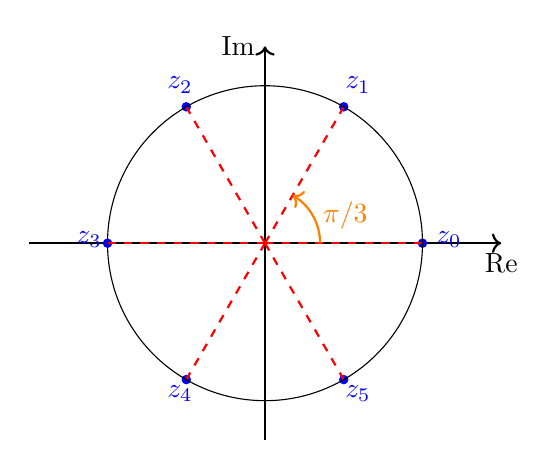
\begin{tikzpicture}
				\draw[thick,->] (-3.0,0) -- (3.0,0) node[below] {$\Re$};
				\draw[thick,->] (0,-2.5) -- (0,2.5) node[left] {$\Im$};
				
				\foreach \angle/\label [count=\k from 0] in {0/$z_0$, 60/$z_1$, 120/$z_2$, 180/$z_3$, 240/$z_4$, 300/$z_5$} {
					\coordinate (z\k) at (\angle:2);
					\draw[fill, blue] (z\k) circle (1.5pt) node[anchor={\angle-180}, shift={(0.05,0.05)}] {\label};
				}
				
				% draw radius
				\draw[dashed, thick, red] (0,0) -- (2,0) node[midway, above left, black] {};
				\draw[dashed, thick, red] (0,0) -- (1,{sqrt(3)}) node[midway, above left, black] {};
				\draw[dashed, thick, red] (0,0) -- (-1,{sqrt(3)}) node[midway, above left, black] {};
				\draw[dashed, thick, red] (0,0) -- (-2,0) node[midway, above left, black] {};
				\draw[dashed, thick, red] (0,0) -- (-1,-{sqrt(3)}) node[midway, above left, black] {};
				\draw[dashed, thick, red] (0,0) -- (1,-{sqrt(3)}) node[midway, above left, black] {};
				
				\draw[->, thick, orange] (.7,0) arc (0:60:.7) node[midway, right, orange] {$\pi/3$};
				\draw (0,0) circle (2);
			\end{tikzpicture}
		\end{center}
		Thus, $z_k=2\exp\of{\frac{k}{3}\pi i}$ with $k\in\set{0,1,2,3,4,5}:$\begin{align*}
			z_0&=2\of{\cos 0+i\sin 0}=2+0i,\\
			z_1&=2\of{\cos\of{\frac{\pi}{3}}+i\sin\of{\frac{\pi}{3}}}=1+\sqrt{3}i,\\
			z_2&=2\of{\cos\of{\frac{2\pi}{3}}+i\sin\of{\frac{\pi}{3}}}=-1+\sqrt{3}i,\\
			z_3&=2\of{\cos\pi+i\sin\pi}=-2+0i,\\
			z_4&=2\of{\cos\of{\frac{4\pi}{3}}+i\sin\of{\frac{4\pi}{3}}}=-1-\sqrt{3}i,\\
			z_5&=2\of{\cos\of{\frac{5\pi}{3}}+i\sin\of{\frac{5\pi}{3}}}=1-\sqrt{3}i.
		\end{align*}
		Note that: \begin{table}[ht!]
			\centering
			\begin{tabular}{c||c|c|c}
				\toprule
				Angle & $\sin(\theta)$ & $\cos(\theta)$ & $\tan(\theta)$ \\
				\midrule
				$0^\circ$ or $0$ & 0 & 1 & 0 \\
				$30^\circ$ or ${\pi}/{6}$ & ${1}/{2}$ & ${\sqrt{3}}/{2}$ & ${\sqrt{3}}/{6}$ \\
				$45^\circ$ or ${\pi}/{4}$ & ${1}/{\sqrt{2}}$ & ${1}/{\sqrt{2}}$ & 1 \\
				$60^\circ$ or ${\pi}/{3}$ & ${\sqrt{3}}/{2}$ & ${1}/{2}$ & $\sqrt{3}$ \\
				$90^\circ$ or ${\pi}/{2}$ & 1 & 0 & undefined \\
				$120^\circ$ or ${2\pi}/{3}$ & ${\sqrt{3}}/{2}$ & $-{1}/{2}$ & $-\sqrt{3}$ \\
				$135^\circ$ or ${3\pi}/{4}$ & ${1}/{\sqrt{2}}$ & $-{1}/{\sqrt{2}}$ & -1 \\
				$150^\circ$ or ${5\pi}/{6}$ & ${1}/{2}$ & $-{\sqrt{3}}/{2}$ & ${\sqrt{3}}/{3}$ \\
				$180^\circ$ or $\pi$ & 0 & -1 & 0 \\
				\bottomrule
			\end{tabular}
			%\caption{Special angles and their sine, cosine, and tangent values}
		\end{table}\\
	\end{proof}
	\vspace{8pt}
	\item Determine whether the following functions are differentiable and holomorphic at $z = 0$.
	\begin{enumerate}
		\item[(a)] $f\of{z}=f\of{x+iy}=\of{x+2y}+i\of{2x+y}$
		\item[(b)] $f\of{z}=\abs{z}^2+z$
		\item[(c)] $f\of{z}=f\of{x+iy}=e^x\cos y+ie^x\sin y$
		\item[(d)] $\displaystyle f\of{z}=f\of{x+iy}=\begin{cases}\displaystyle
			\frac{2x^3-3y^3}{2x^2+3y^2}+i\frac{2x^3+3y^3}{2x^2+3y^2} &:z\neq 0,\\
			0 &:z= 0.
		\end{cases}$
	\end{enumerate}
	\begin{proof}[\sol]
		Note that \begin{align*}
			\text{Complex-differentiable}&\Rightarrow\text{CR-Eq}\\
			\text{Complex-differentiable}&\Leftarrow\text{CR-Eq and $C^1$}\\
		\end{align*}\begin{enumerate}
			\item[(a)] Let $\begin{cases}
				u(x,y)=x+2y,\\
				v(x,y)=2x+y.
			\end{cases}$ Then \[
			u_x=1,\quad u_y=2,\quad v_x=2,\quad\text{and}\quad v_y=1.
			\] Thus $u_x=v_y$ but $u_y\neq -v_x$, that is, it does not hold CR-eqs. Thus $f$ is non-differentiable, and so not holomorphic. 
			\vspace{4pt}
			\item[(b)] Let $z=x+iy$ then $f\of{z}=x^2+y^2+(x+iy)$. Define $\begin{cases}
				u(x,y):=x^2+x+y^2,\\
				v(x,y):=y.
			\end{cases}$ Then \[
			u_x=2x+1,\quad u_y=2y,\quad v_x=0,\quad\text{and}\quad v_y=1.
			\] And so \begin{align*}
				u_x=v_y&\implies 2x+1=1\implies 2x=0,\\
				u_y=-v_x&\implies 2y=0.
			\end{align*} Thus $f$ is differentiable at $z=0$ only. It is not holomorphic.
			\vspace{4pt}
			\item[(c)] Let $\begin{cases}
				u(x,y)=e^x\cos y,\\
				v(x,y)=e^x\sin y
			\end{cases}$ then \[
			u_x=e^x\cos y,\quad u_y=-e^x\sin y,\quad v_x=e^x\sin y,\quad\text{and}\quad v_y=e^x\cos y.
			\] Since $u_x=v_y$ and $u_y=-v_x$, a function $f$ satisfies CR-Eqs and $C^1$. Thus $f$ is differentiable on $\C$ and holomorphic in $\C$. And \[
			f'\of{z}=u_x+iv_x=e^x\cos y+ie^x\sin y=e^{x+iy}=e^z.
			\]
			\vspace{4pt}
			\item[(d)] Note that \textbf{HW\#1}.
		\end{enumerate}
	\end{proof}
	\newpage
	\item For the curve $C:z(t) = 3 + 3e^{it}$ with $0\leq t\leq\pi$, find the $\displaystyle\int_C\conjugate{z}dz$.
	\begin{center}
	\begin{tikzpicture}[scale=1.2]
		\draw[->] (-1,0) -- (7,0) node[right] {$\operatorname{Re}(z)$};
		\draw[->] (0,-1) -- (0,4) node[above] {$\operatorname{Im}(z)$};
		\draw[thick,red] (6,0) arc (0:180:3);
		\node[below left] at (0,0) {$O$};
		\node[below right] at (3,0) {$3$};
		\node[below right] at (6,0) {$6$};
		\node[above left, red] at (3,3) {$D$};
		\node[above left] at (0,3) {$3i$};
		\draw[fill=black] (3,0) circle (0.05);
		\draw[fill=black] (6,0) circle (0.05);
		\draw[fill=black] (0,0) circle (0.05);
		\draw[fill=black] (0,3) circle (0.05);
	\end{tikzpicture}
	\end{center}
	\begin{proof}[\sol]
		Let $\tilde{C}$ be a straight joining origin to $(0,6)$. Define $D:=C+\tilde{C}$. Then \[
		\int_{C+\tilde{C}}\conjugate{z}dz=2i\cdot\of{\text{Area of semi-circle}}=2i\cdot\frac{9\pi}{2}=9\pi i.
		\] Since $\int_{\tilde{C}}\conjugate{z}dz\overset{z(t)=t}{=}\int_0^6\conjugate{t}dt=\int_0^6 tdt=\frac{1}{2}t^2\bigg|_0^6=18$, we have \[
		\int_C\conjugate{z}dz=\int_{C+\tilde{C}}\conjugate{z}dz-\int_{\tilde{C}}\conjugate{z}dz=9\pi -18.
		\]
	\end{proof}
	\vspace{8pt}
	\item Let $C$ be a straight line joining $z_1=0$ to $z_2=1+i$. For $f\of{z}=3z^2+4iz$, find $\int_C f\of{z}dz$.
	\begin{proof}[\sol]
		Note that \[
		f\of{z}=3z^2+4iz=\frac{d}{dz}\left[z^3+2iz^2\right].
		\] Let $F\of{z}:=z^3+2iz^2$. Then \begin{align*}
		\int_Cf\of{z}dz=\int_0^{1+i}f\of{z}dz=F\of{1+i}-F\of{0}&=\of{1+i}^3-2i(1+i)^2-0\\
		&=1+3i+3i^2+i^3-2i(1+2i+i^2)\\
		&=-2+2i+(-2i+4+2i)\\
		&=2+2i.
		\end{align*}
	\end{proof}
	\newpage
	\item Define a principal value of complex exponent as follows: \[
	\pv z^\alpha:=\exp\of{a\Log z}.
	\] Find $\abs{\pv\of{1-i}^{1+i}}$.
	\begin{proof}[\sol]
		Note that \begin{align*}
			\pv (1-i)^{1+i}&=\exp\left[(1+i)\Log(1-i)\right]\\
			&=\exp\left[(1+i)\set{\ln\abs{1-i}+i\Arg\of{1-i}}\right]\\
			&=\exp\left[(1+i)\of{\ln\sqrt{2}-\frac{\pi}{4}i}\right]\\
			&=\exp\left[\of{\ln\sqrt{2}+\frac{\pi}{4}}+i\of{\ln\sqrt{2}-\frac{\pi}{4}}\right].
		\end{align*} Thus, \begin{align*}
		\abs{\pv(1-i)^{1+i}}&=\abs{\exp\of{\ln\sqrt{2}+\frac{\pi}{4}}}\abs{\exp\left[i\of{\ln\sqrt{2}-\frac{\pi}{4}}\right]}\\
		&=\sqrt{2}\exp\of{\frac{\pi}{4}}\quad\because \abs{e^{i\theta}}=1.
	\end{align*}
	\end{proof}
	\vspace{8pt}
	\item Consider the complex function $h\of{z}$ defined as follows: \[
	h\of{z}=h\of{x+iy}=\of{x^3+3xy^2-3x}+i\of{y^3+3x^2y-3y}.
	\]\begin{itemize}
		\item[(a)] Show that $h\of{z}$ is differentiable at all points on $x$-axis.
		\item[(b)] Find all points where $h\of{z}$ is holomorphic.
	\end{itemize}
	\begin{proof}[\sol]
		\begin{itemize}
			\item[(a)]
			Let $\begin{cases}
				u(x,y)=x^3+3xy^2-3x\\
				v(x,y)=y^3+3x^2y-3y
			\end{cases}$ then \[
			\begin{cases}
				u_x=3x^2+3y^2-3\\
				u_y=6xy
			\end{cases},\quad
			\begin{cases}
				v_x=6xy\\
				v_y=3y^2+3x^2-3.
			\end{cases}
			\] Thus, \[\begin{cases}
				u_x=v_y&\\
				u_y=-v_x &\text{if $y=0$ or $x=0$}
			\end{cases}
			\] Therefore, $h$ is complex differentiable on $x=0$ ($y$-axis) or $y=0$ ($x$-axis).
			\vspace{4pt}
			\item[(b)] Consider a $\delta$-neighborhood $N_{\delta>0}(z_0)=\set{z:\abs{z-z_0}<\delta}$ of a point $z_0=x_0+i\cdot 0$ on $y=0$. Thus there is no holomorphic point.
		\end{itemize}
	\end{proof}
	
	\newpage
	\item The curve $C$ is the unit circle $z(t) = e^{it}$ for $0\leq t\leq 2\pi$. Calculate the following integral: \begin{enumerate}
		\item[(a)] $\displaystyle\int_C\frac{2z-10}{z^2-10z}dz$.
		\vspace{4pt}
		\item[(b)] $\displaystyle\int_C\frac{\sinh z}{z^4}dz$.
	\end{enumerate}
	\begin{proof}[\sol]
		Recall that Cauchy integral formula: \[
		f^{(n)}(z_0)=\frac{n!}{2\pi}\oint_C\frac{f\of{z}}{\of{z-z_0}^{n+1}}dz.
		\]
		\begin{itemize}
			\item[(a)] \begin{align*}
				\int_C\frac{2z-10}{z^2-10z}dz&=\oint_C\of{\frac{1}{z}+\frac{1}{z-10}}dz\\
				&=\oint_C\frac{1}{z}dz+\oint_C\frac{1}{z-10}dz\\
				&=2\pi i+0\quad\text{by Cauchy Integral Theorem and Cauchy-Gorusat Theorem}.
			\end{align*}
			\item[(b)] Let $f\of{z}=\sinh z$. Then \[
			f^{(3)}(0)=\frac{3!}{2\pi i}\oint_C\frac{\sinh z}{(z-0)^4}dz=\frac{3}{\pi i}\oint_C\frac{\sinh z}{z^4}dz.
			\] Since $f^{(3)}(z)=\cosh z\Rightarrow f^{(3)}(0)=1$, we have $\displaystyle\int_C\frac{\sinh z}{z^4}dz=\frac{\pi i}{3}$.
		\end{itemize}
	\end{proof}
	\vspace{8pt}
	\item Let the two curves $C_R$ and $C_\rho$ in the complex plane be positively oriented semicircles, defined as follows:
	\[
	C_R: z(t) = Re^{it},\quad  C_\rho: z(t) = \rho e^{it},\quad \of{0\leq t\leq\pi}.
	\] Let the complex function $\displaystyle f(z) = \frac{z^2}{\of{z^2+1}^2}$. 
	\begin{center}
		\begin{tikzpicture}
			\draw[thick,->] (-6.0,0) -- (6.0,0) node[below] {$\Re$};
			\draw[thick,->] (0,-.5) -- (0,5) node[left] {$\Im$};
			
			\node[below] at (2,0) {$\rho$};
			\node[below] at (4,0) {$R$};
			\node[below] at (-2,0) {$-\rho$};
			\node[below] at (-4,0) {$-R$};
			\draw[fill=red] (2,0) circle (0.05);
			\draw[fill=red] (4,0) circle (0.05);
			\draw[fill=red] (-2,0) circle (0.05);
			\draw[fill=red] (-4,0) circle (0.05);
			
			\draw[->, thick, red] (2,0) arc (0:180:2) node[above left, black] {$C_\rho$};
			\draw[->, thick, red] (4,0) arc (0:180:4) node[above left, black] {$C_R$};
			%\draw[->, thick, red] (2,0) arc (0:90:2)
			%\draw[->, thick, red] (4,0) arc (0:90:4)
			%\draw (0,0) circle (2);
		\end{tikzpicture}
	\end{center}
	\vspace{4pt}
	\begin{enumerate}
		\item[(a)] Prove the following inequality when $R=3$: \[
		\abs{\int_{C_R}f\of{z}dz}<\frac{1}{2}\pi.
		\] As the radius $R$ approaches infinity $\of{R\to\infty}$, where does the integral value converge?
		\item[(b)] Prove the following inequality when $\rho = 1/3$:
		\[
		\abs{\int_{C_\rho}f\of{z}dz}<\frac{1}{16}\pi.
		\] As the radius $\rho$ approaches zero $\of{\rho\to 0}$, where does the integral value converge?
	\end{enumerate}
	\begin{proof}[\sol]
	\begin{enumerate}
			\item[(a)] For $\abs{z}=3$, we have $\abs{z^2+1}\geq\abs{\abs{z}^2-1}=8$. Then \[
			\abs{f\of{z}}=\frac{\abs{z}^2}{\abs{z^2+1}^2}\leq\frac{9}{64}.
			\] Thus \[
			\abs{\int_{C_R}f\of{z}dz}\leq\max_{z\in C_R}\abs{f\of{z}}\int_{C_R}\abs{dz}\leq\frac{9}{64}\cdot3\pi=\frac{27}{64}\pi<\frac{1}{2}\pi.
			\] Suppose that $R\to\infty$ then \[
			\abs{\int_{C_R}f\of{z}dz}\leq\frac{R^2}{\of{R^2-1}^2}\cdot\pi R=\frac{\pi R^3}{\of{R^2-1}^2}\to 0.
			\]
			\vspace{4pt}
			\item[(b)] For $\abs{z}=1/3$, we have $\abs{z^2+1}\geq 1-\abs{z}^2=1-\rho^2=8/9$. Then \[
			\abs{f\of{z}}=\frac{\abs{z}^2}{\abs{z^2+1}^2}\leq\frac{\rho^2}{(1-\rho^2)^2}=\frac{1/9}{\of{8/9}^2}=\frac{9}{64}.
			\] Thus, \[
			\abs{\int_{C_\rho}f\of{z}dz}\leq\max_{z\in C_\rho}\abs{f\of{z}}\int_{C_\rho}\abs{dz}\leq\frac{9}{64}\cdot\frac{1}{3}\pi=\frac{3}{64}\pi<\frac{1}{16}\pi.
			\] Suppose that $\rho\to 0$ then \[
			\abs{\int_{C_\rho}f\of{z}dz}\leq\frac{\rho^2}{\of{1-\rho^2}^2}\cdot\pi \rho=\frac{\pi \rho^3}{\of{1-\rho^2}^2}\to \frac{0}{1}=0.
			\]
		\end{enumerate}
	\end{proof}
	
	\newpage
	\item Show that an entire function $f$ becomes a constant function if it satisfies the following condition: \[
	\abs{f\of{z}}\geq 1,\quad z\in\C.
	\]
	\begin{proof}[\sol]
		We use Liouville's theorem: ``bounded and entire $\Rightarrow$ constant''. Define an entire function \[
		g\of{z}:=\frac{1}{f\of{z}}.
		\] Then $\abs{g\of{z}}=\frac{1}{\abs{f\of{z}}}\leq 1$, \ie, $g$ is bounded. By Liouville's theorem, $g$ be a constant function, and hence $f$ be a constant.
	\end{proof}
	\vspace{8pt}
	\item For an entire function $f$ satisfying the following condition: \[
	\abs{f\of{z}}\leq 3\abs{z},\quad z\in\C,
	\] \begin{enumerate}
		\item[(a)] Show that $f^{(n)}(z) = 0$ ($n\geq 2$) for all points $z$.
		\item[(b)] Demonstrate that a function satisfying this condition is a linear polynomial, \ie, $f(z) = az + b$.
	\end{enumerate}\begin{proof}[\sol]
		\begin{itemize}
			\item[(a)] By the Cauchy integral formula, \begin{align*}
				\abs{f^{(2)}\of{z_0}}=\abs{\frac{2!}{2\pi i}\oint_{C_R}\frac{f\of{z}}{\of{z-z_0}^3}dz}&=\frac{1}{\pi}\abs{\oint_{C_R}\frac{f(z)}{(z-z_0)^3}dz}\\
				&\leq\frac{1}{\pi}\cdot\max_{z\in C_R}\frac{\abs{f\of{z}}}{\abs{z-z_0}^3}\cdot 2\pi R\\
				&\leq 2R\cdot\frac{3R}{\of{R-\abs{z_0}}^3}\\
				&=\frac{6R}{\of{R-\abs{z_0}}^3}\\
				&\to 0\quad\text{as $R\to\infty$}.
			\end{align*} Thus, $f^{(n)}=0$ for all $n\geq 2$.
			\vspace{4pt}
			\item[(b)] \[
			f^{(2)}(z)=0\implies f^{(1)}(z)=c\in\C\implies f(z)=az+b\ (\text{linear}).
			\]
		\end{itemize}
	\end{proof}
\end{enumerate}


\footer{Department of Information Security, Cryptography and Mathematics, Kookmin University}
\end{document}
